\section{Auswertung}
\label{sec:Auswertung}


In Tabelle \ref{tab:tabelle1} ist der experimentell bestimmte Wert $U_out$ abhängig von $\increment \varphi$ aufgelistet.
Zudem wird ein, mit Gleichung \ref{eqn:cos} berechneter theoretischer Wert, in die Tabelle eingetragen.
Zudem wird die Abweichung $A_{e,t}$ vom theoretischen Wert mit 
\begin{equation}
  A_{n,m}=\Biggl|\frac{U_{n}-U_{m}}{U_{m}}\Biggr|
  \label{eqn:Abweichung}
\end{equation}
berechnet.
Außerdem wurden die Messung mit einem Rauschsignal ebenfalls in die Tabelle eingetragen.
Hier wurde mit Formel \ref{eqn:Abweichung} die Abweichung $A_{N,e}$vom Wert mit Rauschen zu dem ohne gebildet.


\begin{table}
  \centering
  \caption{Aufgelistet ist die gemessene Ausgangsspannung abhängig von Phasenverschiebung der Referenzspannung. 
  Zudem ist ein theoretischer Wert, sowie die Abweichung zu diesem, eingetragen.
  Außerdem wurden die Werte, die bei einem Rauschen gemessen wurden, eingetragen und die Abweichung zu den Werten ohne Rauschen bestimmt.
  }
  \label{tab:tabelle1}
  \sisetup{table-format=1.1, per-mode=reciprocal}
  \begin{tblr}{
      colspec = {S[table-format=3.0] S[table-format=1.2] S[table-format=1.2] S[table-format=2.2] S[table-format=1.2] S[table-format=1.2]},
      row{1} = {guard, mode=math},
   %   vline{4} = {2}{-}{text=\clap{$\pm$}},
    }
    \toprule
    \varphi \mathbin{/} \unit{\degree} & U_{out} \mathbin{/} \unit{\volt}  & U_{out,t} \mathbin{/} \unit{\volt} & A_{e,t} \mathbin{/} \unit{\percent} & U_{out,N} \mathbin{/} \unit{\volt} & A_{N,e} \mathbin{/} \unit{\percent}\\
    \midrule
    0     &  2.96   &  2.96 &   0.00  &  2.96 &  0.00   \\
    45    &  2.64   &  2.09 &  26.13  &  2.72 &  3.03   \\
    90    &  0.96   &  0.00 &  X      &  0.96 &  0.00   \\
    135   & -1.04   & -2.09 &  50.31  & -1.04 &  0.00   \\
    180   & -2.40   & -2.96 &  18.92  & -2.48 &  3.33   \\
    225   & -2.08   & -2.09 &   6.23  & -2.16 &  3.85   \\
    270   & -0.48   &  0.00 &  X      & -0.48 &  0.00   \\
    315   &  1.60   &  2.09 &  23.56  &  1.52 &  5.00   \\
    360   &  2.96   &  2.96 &   0.00  &  2.96 &  0.00   \\
    \bottomrule
  \end{tblr}
\end{table}

Die Werte für die Ausgangsspannung werden in \ref{fig:plot} ohne Noise und in \ref{fig:plot1}, mit der passenden Cosinusfunktion, abhängig zur Phasenverschiebung aufgetragen.

\begin{figure}[H]
  \centering
  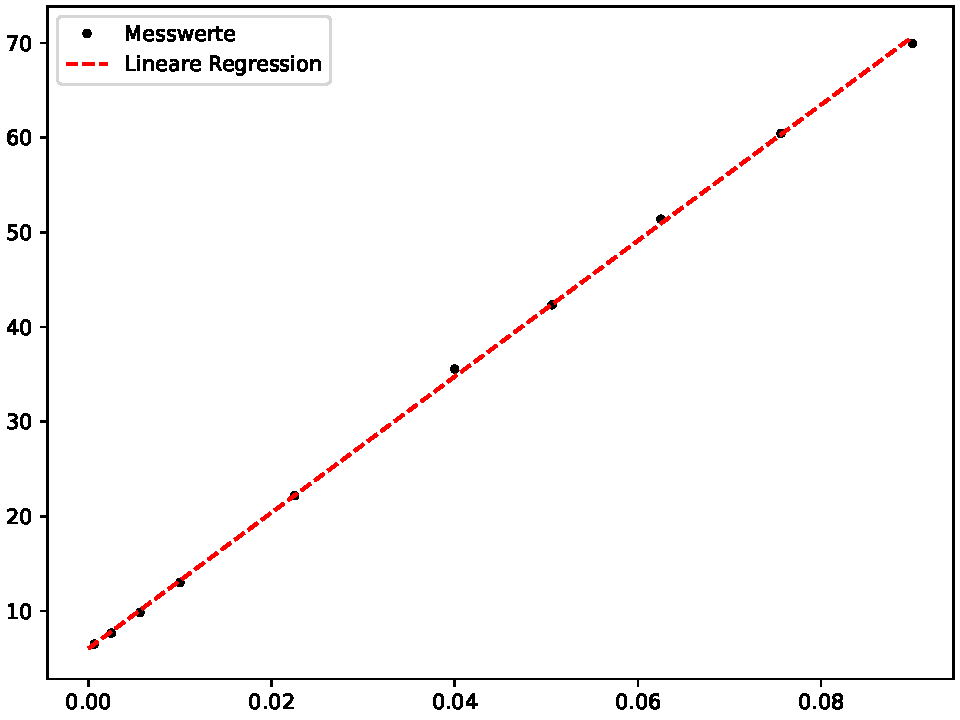
\includegraphics[height=5cm]{plot.pdf}
  \caption{Aufgetragen ist die Ausgangsspannung abhängig von der Zeit ohne Noise.}
  \label{fig:plot}
\end{figure}

\begin{figure}[H]
  \centering
  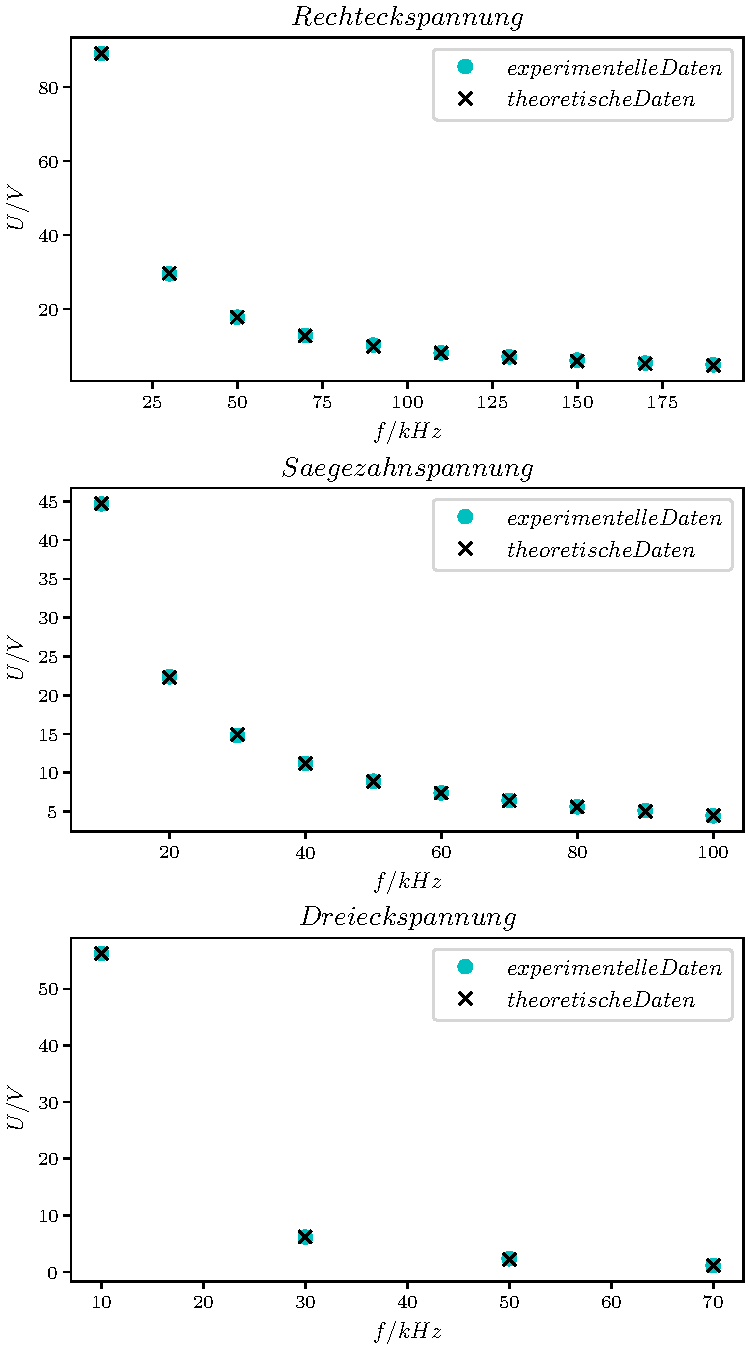
\includegraphics[height=5cm]{plot1.pdf}
  \caption{Aufgetragen ist die Ausgangsspannung abhängig von der Zeit mit Noise.}
  \label{fig:plot1}
\end{figure}



Für verschiedene Werte von $\increment \varphi$ von 0° bis 360°, mit Abständen von jeweils 90°, wird das Ausgangssignal in den Abbildungen \ref{fig:phi0} bis \ref{fig:phi360} dargestellt.
Dabei handelt es sich um die Ausgangspannung abhängig von der Zeit. 
Für das Signal mit eingeschaltetem Noise-Generator wurde dies wiederholt.
Die dabei entstandenen Verläufe wurden in den Abbildungen \ref{fig:n_phi0} bis \ref{fig:n_phi360} dargestellt.

\begin{figure}[H]
  \centering
  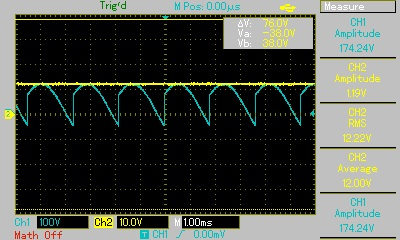
\includegraphics[height=5cm]{Bilder/phi0.jpg}
  \caption{Abgebildet ist das Spannung zu Zeit Diagramm des des Lock-In-Verstärkers ohne Noise mit einer Phasenverschiebung von 0.}
  \label{fig:phi0}
\end{figure}

\begin{figure}[H]
  \centering
  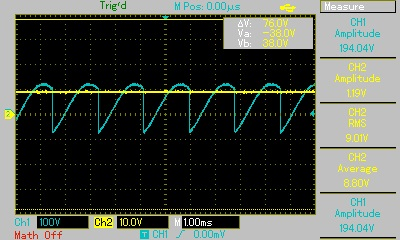
\includegraphics[height=5cm]{Bilder/phi90.jpg}
  \caption{Abgebildet ist das Spannung zu Zeit Diagramm des des Lock-In-Verstärkers ohne Noise mit einer Phasenverschiebung von 90°.}
  \label{fig:phi90}
\end{figure}

\begin{figure}[H]
  \centering
  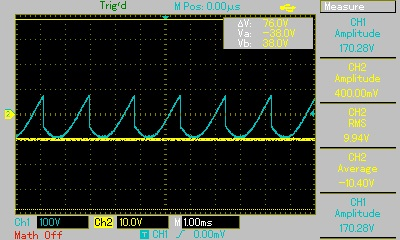
\includegraphics[height=5cm]{Bilder/phi180.jpg}
  \caption{Abgebildet ist das Spannung zu Zeit Diagramm des des Lock-In-Verstärkers ohne Noise mit einer Phasenverschiebung von 180°.}
  \label{fig:phi180}
\end{figure}

\begin{figure}[H]
  \centering
  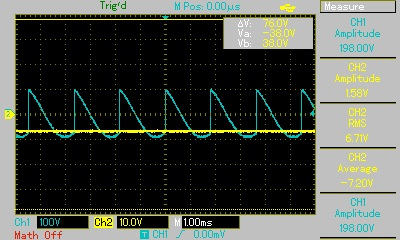
\includegraphics[height=5cm]{Bilder/phi270.jpg}
  \caption{Abgebildet ist das Spannung zu Zeit Diagramm des des Lock-In-Verstärkers ohne Noise mit einer Phasenverschiebung von 270°.}
  \label{fig:phi270}
\end{figure}

\begin{figure}[H]
  \centering
  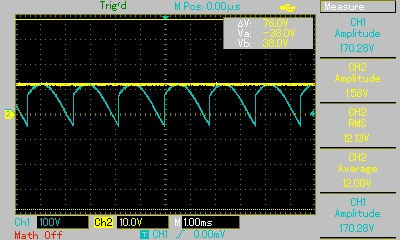
\includegraphics[height=5cm]{Bilder/phi360.jpg}
  \caption{Abgebildet ist das Spannung zu Zeit Diagramm des des Lock-In-Verstärkers ohne Noise mit einer Phasenverschiebung von 360°.}
  \label{fig:phi360}
\end{figure}

\begin{figure}[H]
  \centering
  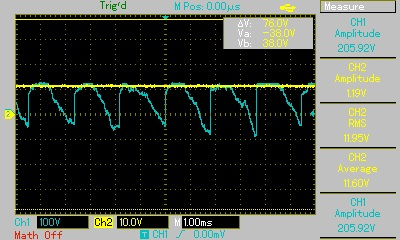
\includegraphics[height=5cm]{Bilder/n_phi0.jpg}
  \caption{Abgebildet ist das Spannung zu Zeit Diagramm des des Lock-In-Verstärkers mit Noise mit einer Phasenverschiebung von 0.}
  \label{fig:n_phi0}
\end{figure}

\begin{figure}[H]
  \centering
  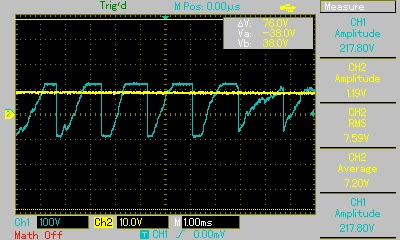
\includegraphics[height=5cm]{Bilder/n_phi90.jpg}
  \caption{Abgebildet ist das Spannung zu Zeit Diagramm des des Lock-In-Verstärkers mit Noise mit einer Phasenverschiebung von 90°.}
  \label{fig:n_phi90}
\end{figure}

\begin{figure}[H]
  \centering
  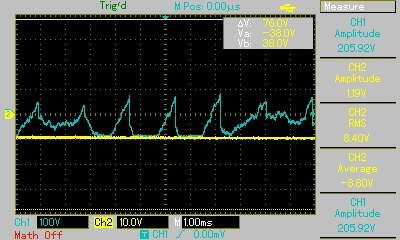
\includegraphics[height=5cm]{Bilder/n_phi180.jpg}
  \caption{Abgebildet ist das Spannung zu Zeit Diagramm des des Lock-In-Verstärkers mit Noise mit einer Phasenverschiebung von 180°.}
  \label{fig:n_phi180}
\end{figure}

\begin{figure}[H]
  \centering
  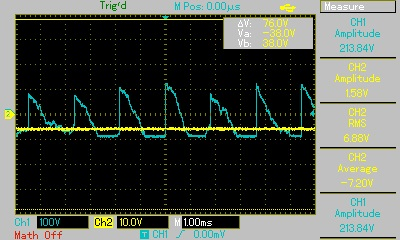
\includegraphics[height=5cm]{Bilder/n_phi270.jpg}
  \caption{Abgebildet ist das Spannung zu Zeit Diagramm des des Lock-In-Verstärkers mit Noise mit einer Phasenverschiebung von 270°.}
  \label{fig:n_phi270}
\end{figure}

\begin{figure}[H]
  \centering
  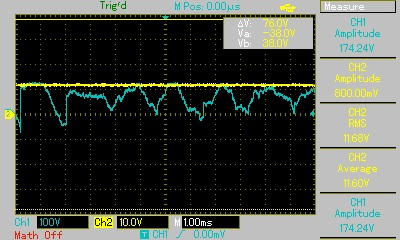
\includegraphics[height=5cm]{Bilder/n_phi360.jpg}
  \caption{Abgebildet ist das Spannung zu Zeit Diagramm des des Lock-In-Verstärkers mit Noise mit einer Phasenverschiebung von 360°.}
  \label{fig:n_phi360}
\end{figure}

\subsection{Photodetektorschaltung}
In Tabelle \ref{tab:tabelle2} ist die gemessene Spannung in Abhängigkeit zum Abstand r zwischen Leucht- und Photodiode eingetragen.
Graphisch dargestellt ist dies ebenfalls in Abbildung \ref{fig:plot2}.

\begin{table}
  \centering
  \caption{Aufgelistet ist die Ausgangsspannung abhängig von der Entfernung der Leuchtdiode von der Photodiode.
  }
  \label{tab:tabelle2}
  \sisetup{table-format=1.1, per-mode=reciprocal}
  \begin{tblr}{
      colspec = {S[table-format=3.0] S[table-format=1.2] S[table-format=1.2] S[table-format=2.2] },
      row{1} = {guard, mode=math},
   %   vline{4} = {2}{-}{text=\clap{$\pm$}},
    }
    \toprule
    r \mathbin{/} \unit{\centi\meter} & U_{out} \mathbin{/} \unit{\volt}  &  r \mathbin{/} \unit{\centi\meter} &  U_{out} \mathbin{/} \unit{\volt} \\
    \midrule
       2    &     14.4  &    62   &    5.6  \\   
       7    &     14.4  &    67   &    5.6  \\
      12    &     13.6  &    72   &    4.8  \\
      17    &     12.0  &    77   &    4.8  \\
      22    &     12.0  &    82   &    4.8  \\
      27    &     12.0  &    87   &    4.8  \\
      32    &     10.4  &    92   &    4.8  \\
      37    &      9.6  &    97   &    4.0  \\
      42    &      8.0  &   107   &    4.0  \\
      47    &      7.2  &   117   &    4.0  \\
      52    &      6.4  &   127   &    4.0  \\
      57    &      6.4  &   137   &    3.2  \\
    \bottomrule
  \end{tblr}
\end{table}


\begin{figure}[H]
  \centering
  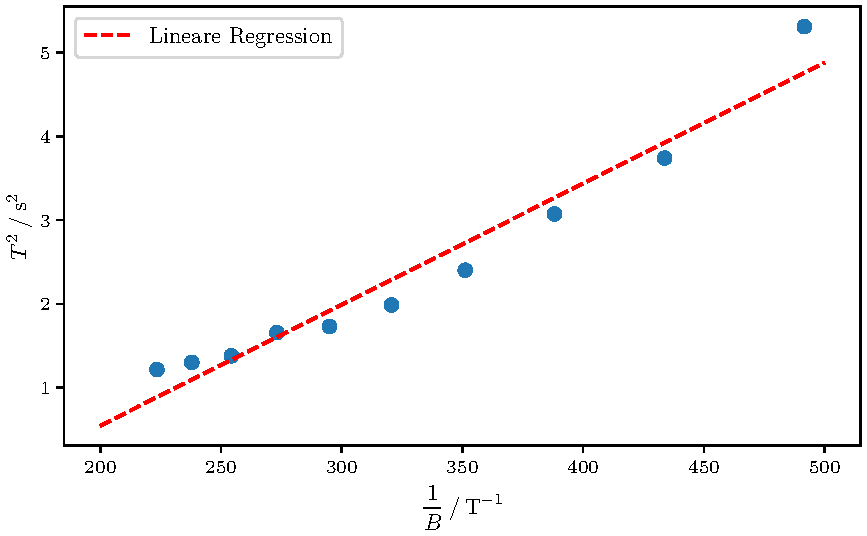
\includegraphics[height=5cm]{plot2.pdf}
  \caption{Aufgetragen ist die Ausgangsspannung in Abhängigkeit zur Entfernung der Leuchtdiode zur Photodiode.}
  \label{fig:plot2}
\end{figure}


